\documentclass{article}

\usepackage[letterpaper, portrait, margin=1.5in]{geometry}

\usepackage{fancyhdr}
\usepackage{ragged2e}
\usepackage{graphicx}
\usepackage{caption}
\usepackage{amsmath}
\usepackage{rotating}

\usepackage{listings}
\usepackage{color}

\definecolor{dkgreen}{rgb}{0,0.6,0}
\definecolor{gray}{rgb}{0.5,0.5,0.5}
\definecolor{mauve}{rgb}{0.58,0,0.82}

\lstset{frame=tb,
  language=Java,
  aboveskip=3mm,
  belowskip=3mm,
  showstringspaces=false,
  columns=flexible,
  basicstyle={\small\ttfamily},
  numbers=none,
  numberstyle=\tiny\color{gray},
  keywordstyle=\color{blue},
  commentstyle=\color{dkgreen},
  stringstyle=\color{mauve},
  breaklines=true,
  breakatwhitespace=true,
  tabsize=4
}

\setcounter{secnumdepth}{1}

\usepackage{chngcntr}
\counterwithin{figure}{section}

\renewcommand*{\thepage}{C\arabic{page}}

\pagestyle{fancy}
\lhead{ACME Robotics}
\chead{\#8367}
\rhead{\ifcontents Contents \else Week \thesection \fi}

\newif\ifcontents
\contentstrue

\makeatletter
\renewcommand{\@seccntformat}[1]{}
\makeatother
\begin{document}
\subsection{Set up the UI for the pre-scouting app}
%! Move on to the next part of the prescouting app which is to set up the UI.
Emma started working on the next part of the prescouting app which is to create a UI. Emma had some experience with creating UIs before as she worked on the scouting app last year. First, she sketched out the design of the UI and everything she would need to display the data, as you can see in Fig \ref{fig:sketch}. 

\begin{figure}
    \centering
    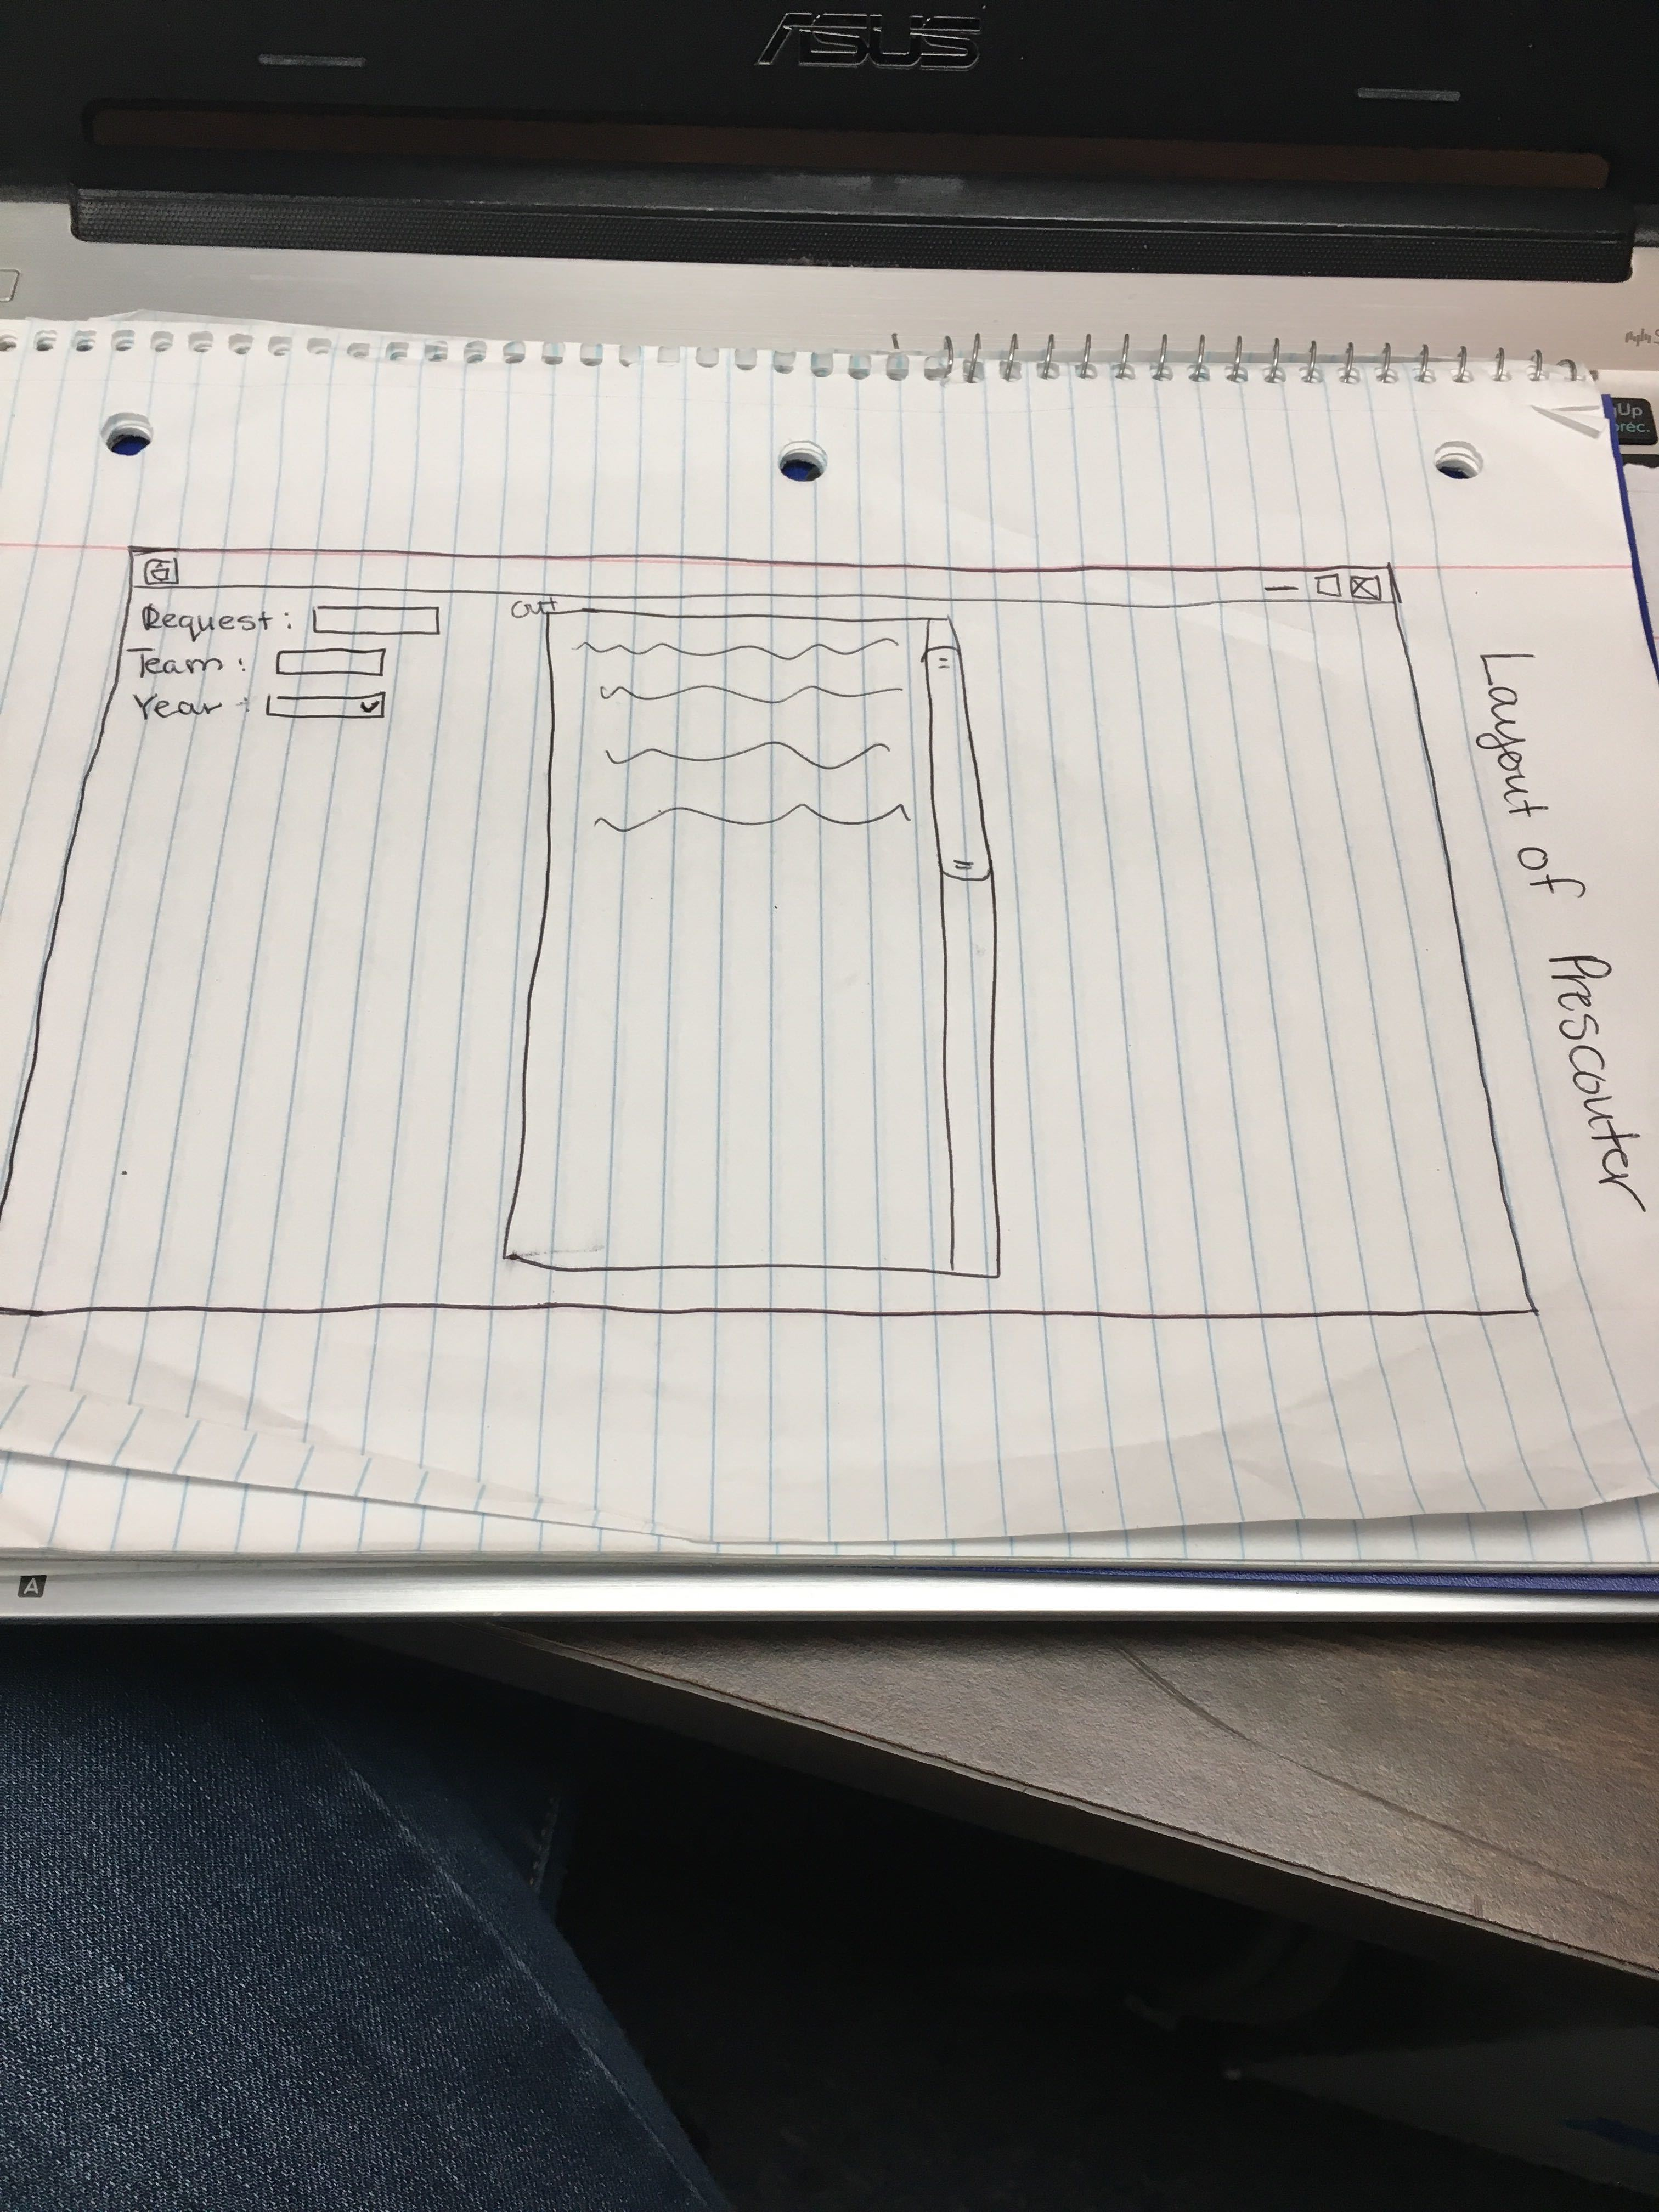
\includegraphics[width=.6 \textwidth]{24_02-11/images/sketchofUI.JPG}
    \caption{Sketch of what UI will look like}
    \label{fig:sketch}
\end{figure}

Next, Emma set to work identifying which components she needed to use to complete the UI. She decided for the request and the team number, she would use TextFields. For the year, she would use a Choice component that would allow the user to select a preset year. She used a Button for the submit button. Finally, she decided to make a Panel on top of her Frame in order to section off the TextArea were the data would be printed from the rest of the screen. 

Now, Emma needed to go about making this UI a reality and actually function properly. She began by setting up the aesthetic parts of the UI (Frame, TextFields, etc). Then she started to figure out how to get the submit button to actually do something. She decided to use an ActionListener for this. An ActionListener is how you tell in Java f a button has been pressed or not. If it has, an action occurs after that. That action that takes place after Emma's submit button is pressed is an if else statement figures out what is in the request TextField and what is in the team number field in order to piece together the URL. She managed to get that working, and is now trying to figure out how to send the GET request once the button has been pressed. Above is the current design the UI, as seen in Fig \ref{fig:UI}.

\begin{figure}
    \centering
    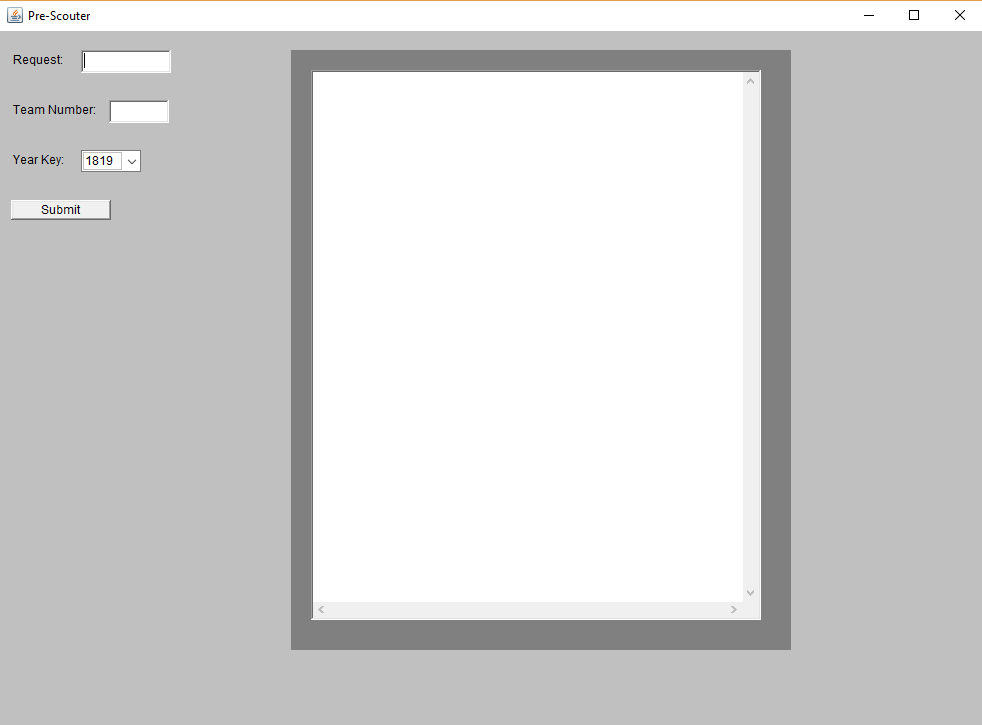
\includegraphics[width=.6 \textwidth]{24_02-11/images/prescoutingapp.png}
    \caption{Design of UI}
    \label{fig:UI}
\end{figure}

\subsection{Write tracking omni code}
%!
To use the omnidirectional tracking wheels installed on the robot Kelly needed to write software to translate their movements into robot movements. The kinematics to transform a relative robot pose update to a field pose up date could be reused from the existing localization code that used the drive motors, so the task was to translate tracking wheel deltas and a heading delta reported by the imu into a robot pose delta. 

Because the drivetrain is holonomic, software assumes that the robot moves with constant positional and heading velocity each update cycle, rather than the traditional twists used by differential drives. 
After drawing a diagram of the paths taken by two tracking wheels during a robot update, Kelly decided that the best course of action would be to first determine what part of each tracking omni delta was accounted for by the heading delta, and then transform the resulting vector from tracking omni space into robot space. 

Accounting for the portion of a tracking omni delta caused by a heading delta is relatively simple. Given a heading delta $\theta$, the linear distance reported by a tracking omni will be $r \theta \sin\alpha$, where r is the distance from the tracking omni to the center of rotation of the robot and $\alpha$ is the angle between the radius and the axis of the tracking omni. While this value could be theoretically determined, Kelly doubted it would be accurate enough to base all robot localization off of, so they decided to determine it empirically. Because the value would be determined empirically, a new coefficient, $k$, can be defined to equal $r \sin\alpha$, eliminating the need to empirically determine more than one constant.

Kelly wrote an opmode to turn the robot a set angle, and then measure the distance reported by each tracking omni. By dividing the distance reported by the heading delta reported by the imu, they empirically determined $k$. They found that $k$ was equal to 3500 ticks per radian for the axial tracking wheel, and zero for the lateral wheel. 

The next step was to convert the two distances traveled by the tracking wheels into the robot coordinate system. This is a very simple problem if the tracking wheels are orthogonal to the robot, one of them is the x component and one of them is the y, and is still very simple if they are orthogonal to each other but rotated relative to the robot, because the vector representing their movement can just be rotated by their angle relative to the robot. However, the general case, for two tracking wheels oriented in arbitrary directions, proved to be much more difficult. 

After a couple naive approaches that involved rotating vectors representing the vectors representing each wheel individually, and constructing equations that passed and were tangent to the vectors and then solving the system, Kelly came to the realization that the same general concepts used in all holonomic wheels could be applied. Most importantly, the dot product of a vector representing robot movement and a unit vector pointing in the direction of the rollers of a wheel is equal to the distance traveled by the rollers. If $\vec{r}$ is the robot position delta, and $\hat{a}$ and $\hat{b}$ are the unit vectors in the direction of the a and b rollers respectively, then $\vec{r} \cdot \hat{a} = |\vec{a}|$ and $\vec{r} \cdot \hat{b} = |\vec{b}|$. By rewriting this as matrix multiplication the following equation results: 

$$\begin{bmatrix} |\vec{a}| & |\vec{b}| \end{bmatrix}^\top = \begin{bmatrix} \hat{a_x} & \hat{a_y} \\ \hat{b
x} & \hat{b_y} \end{bmatrix} \vec{r}^\top$$

and after solving for $\vec{r}$:

$$\vec{r}^\top = \begin{bmatrix} \hat{a_x} & \hat{a_y} \\ \hat{b
x} & \hat{b_y} \end{bmatrix}^{-1}  \begin{bmatrix} |\vec{a}| & |\vec{b}| \end{bmatrix}^\top $$

To actually compute this, the inverse of the unit vectors are derived from angles representing the direction the rollers point, and the inverse matrix is pre-computed, and then each row represented as a vector, so the resulting vector can be represented as two dot products. This small utility class encapsulates this math:

\begin{lstlisting}[language=Java]
public class TrackingWheelKinematics {

    private Vector2d r0, r1;

    public TrackingWheelKinematics (double a0, double a1) {
        if (a0 == a1) throw new IllegalArgumentException("you can't point them in the same direction silly!!!");
        double a = Math.cos(a0);
        double b = Math.sin(a0);
        double c = Math.cos(a1);
        double d = Math.sin(a1);
        double determinant = a*d - b*c;
        r0 = new Vector2d(d, -b).div(determinant);
        r1 = new Vector2d(-c, a).div(determinant);
    }

    public Vector2d transform (Vector2d dist) {
        return new Vector2d(r0.dot(dist), r1.dot(dist));
    }

}
\end{lstlisting}


\end{document}
